\section{Room assistant}\label{sec:room-assistant}

Room Assistant zpřístupňuje komunikaci mezi systémem Home Assistant a službou Room Driver.\newline
S Home Assistantem je komunikace realizována pomocí MQTT(\ref{sec:mqtt}) a s Room driverem pomocí HTTP protokolu.
Tato služba zpřístupňuje do systému Home Assistant data o teplotě a vlhkosti a Home Assistant přes ni ovládá světlo a dvířka.
Při vývoji, ale i při provozu si můžeme zprávy prohlížet pomocí klientských aplikací (obrázek \ref{fig:homeassistant_input_data_mqtt}).

\begin{figure}[h]
    \centering
    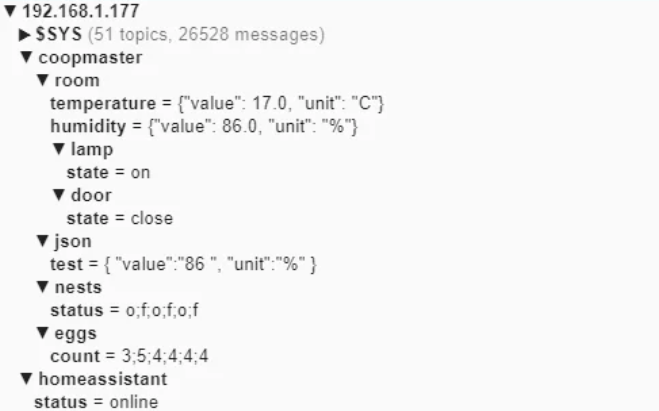
\includegraphics[width=0.8\textwidth]{img/homeassistant_input_data_mqtt}
    \caption{Prohlížeč zpráv uložených na MQTT serveru.}
    \label{fig:homeassistant_input_data_mqtt}
\end{figure}


\subsection*{Popis algoritmu}
Po odstartování služby se stane hned několik věcí.
Jako první naběhnou MQTT subscribery pro přijímání příkazů ze systému Home Assistant.
Jeden přijímá příkazy pro dvířka, druhý pro světlo.
Vytvoří se vlastně instance dvou tříd LampTimeChecker a DoorTimeChecker. \newline
Tyto instance mají každá svou instanci třídy NestMQTTClient, která zaobaluje základní funkcionalitu ohledně používání protokolu MQTT.
NestMQTTClient zaobaluje metody pro publikování a odebírání zprávy, připojení a odpojení od MQTT brokeru, reakci na navázané spojení s MQTT brokerem a reakci na odebrání nové zprávy.
LampTimeChecker odebírá topic coopmaster/room/lamp/cmnd  a zpracovává zprávu pokud je jejím obsahem "on" nebo "off".
Na základě přijatého obsahu zprávy se zavolá statická metoda call\_room\_driver\_command() třídy driver\_client, aby odeslala příslušný příkaz do Room Driveru na endpoint, který je předáván jako parametr.
DoorTimeChecker funguje stejně jako NestMQTTClient, ale odebírá topic coopmaster/room/door/cmnd  a reaguje pokud je obsah MQTT zprávy "open" nebo "close".\newline
Po startu se rozběhne BackgroundScheduler, který má za úkol vždy po uplynutí 5 vteřin spustit nový běh akce pro aktualizování stavů z řídící jednotky.
Podmínkou pro spuštění nového běhu jobu je, že předchozí běh je dokončen.
Tuto funkci má již v sobě implementovanou scheduler z knihovny APScheduler, který využívám.
Akce pro aktualizaci obsahuje jednu metodu a to detect\_hardware\_state().
Tato metoda nejdříve stáhne data z Room Driveru.
Následně načte z konfigurace topic pro stav dvířek, stav světla, teplotu a vlhkost.
Dále jsou pak data z Room Driveru zveřejněna na téma daná kofigurací, odkud je přijímá systém Home Assistant a vizualizuje je.

